\documentclass[]{article}
\usepackage[T1]{fontenc}
\usepackage[top=1in, bottom=1in, left=1in, right=1in]{geometry}
\usepackage{commath,amsmath,amssymb,amsfonts}
\usepackage{algorithmic}
\usepackage{graphicx}
\usepackage{multirow}
\graphicspath{{./images/}}
\usepackage{textcomp}
\usepackage{xcolor}
\usepackage{tikz}
\usepackage[backend=biber, sorting=none]{biblatex}
\usepackage[hidelinks]{hyperref}

\renewcommand{\theenumi}{\alph{enumi})}

%uncomment below line to use reference file
%\addbibresource{references.bib}

%opening
\title{Individual Exercises}
\author{Benjamin Russell, \textit{fdmw97}}
%\date{}

\begin{document}

\maketitle

\section*{Exercise 1}
\section*{Exercise 2}
\begin{enumerate}
	\item When $n$ is very large $R$ is approaching $r$
	\item
	Let $B$ be the set of all bids i.e. 
	\[B=\left\{b_1,b_2,...,b_{n-1},b_n \right\}\]
	Where $b_i$ is the bid of player $i \in [1,n]$.
	The maximum bid $\max(B)$ is $b_n$ as $b_n > r > 1$ by the problem definition.
	Therefore $R=E[\max(B\setminus\{b_n\})]$ i.e. the expected maximum of all bids less than $b_n$.
	\[
	\text{Let}\ B'=B\setminus\{b_n\}
	\]
	So $R=E[\max(B')]$, if any $b\in B'$ bids $r$ then $\max(B')$ is necessarily $r$ as $r>1$ as per the problem definition, else $\max(B')$ is $1$.\\
	We can now model $B'$ using a binomial distribution $B(n-1, 0.5)$ where a success is bidder $b_i$ bidding $r$. Let $X\sim B(n-1,0.5)$ be a discrete random variable representing the number of successes in $n-1$ bidders.
	\begin{align*}
		P(X\geq 1) &= 1-P(X=0) \\
		&= 1-\binom{n-1}{0}\times0.5^0\times0.5^{n-1} \\
		&= 1-0.5^{n-1}
	\end{align*}
This gives the probability that at least $1$ bidder from $B'$ bids $r$ therefore by taking the limit to infinity we can determine $R$ for very large $n$.
\[
\lim_{n \to \infty}  P(x\geq 1) = \lim_{n \to \infty} 1-0.5^{n-1} = 1-0 = 1
\]
This means as $n$ approaches $\infty$, $P(\max(B')=r)=1$ and $P(\max(B')=1)=0$ therefore
\[
	E[\max(B')]=1\times r + 0 \times 1 = r
\]
so $R=E[\max(B')] = r$
\end{enumerate}
\section*{Exercise 3}
\begin{enumerate}
	\item
	Mary's preferences $=u_M$: \\
	$u_M(B,W)=2, u_M(C,J)=1, u_M(C,W)=0, u_M(B,J)=0$\par
	Alice's preferences $=u_A$:\\
	$u_A(C,J)=2, u_A(B,W)=1, u_A(C,W)=0, u_A(B,J)=0$
	\item
	\begin{tabular}[t]{c c | c c}
		 \multicolumn{2}{c}{}& \multicolumn{2}{c}{Alice} \\
		& & W & J \\
		\cline{2-4}
		\multirow{2}{4ex}{Mary} & C & $(0,0)$ & $(1,2)$\\
		& B & $(2,1)$ & $(0,0)$
	\end{tabular}
	\item
	~\\
	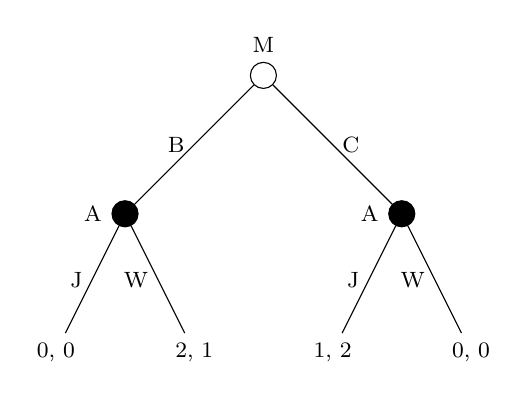
\begin{tikzpicture}[
		round/.style={circle,draw,minimum size=1pt},
		filled/.style={circle, draw, fill=black, minimum size=1pt},
		sibling distance        = 10em,
		level distance          = 5em,
		every node/.style       = {font=\footnotesize}
		]
		\node[round,label=above:M]{}
		child{node[filled,label=left:A]{}[sibling distance=5em]
				child{node[]{0, 0}
				edge from parent node[left]{J}} 
				child{node[]{2, 1}
				edge from parent node[left]{W}}
		edge from parent node[left]{B} }
		child{node[filled,label=left:A]{}[sibling distance=5em]
				child{node[]{1, 2}
				edge from parent node[left]{J}}
				child{node[]{0, 0}
				edge from parent node[left]{W}}
		edge from parent node[right]{C}};
	\end{tikzpicture}
\end{enumerate}
%uncomment below line to print bilbliography
%\printbibliography
\end{document}
